\section{Мета роботи}
Закріпити знання про алгоритми пошуку, що потребують
додаткової пам’яті; набути навичок виконання операцій пошуку із
використанням таблиць прямого доступу, довідників та хешованих таблиць.

\section{Хід роботи}
Початкові дані містяться у текстовому файлі. Прочитати файл,
створити таблицю прямого доступу або хеш-таблицю відповідно до
завдання з табл. 10.1. Перевірити працездатність створених таблиць на
прикладі операцій пошуку.\\

Порівняти час пошуку із використанням створених таблиць та простих
алгоритмів пошуку з лабораторної роботи 4. Для кожного з алгоритмів
визначити кількість порівнянь у наборі даних з різною кількістю елементів
(20, 1000, 5000, 10000, 50000), визначити час пошуку, заповнити таблицю за
формою табл. 10.2, побудувати графіки, зробити висновки.\\

\textbf{Моє завдання:} \\

Дані: Ідентифікаційний код, ім’я користувача мережі, Е-mail адреса.\\
Таблиця: Хеш-таблиця з розподіленими ланцюжками переповнень.\\
Хеш-функція: Функція серединии квадрата та ділення за модулем.\\
Ключ: Ідентифікаційний код.

\clearpage
\subsection{Реалізація хеш-таблиці з розподіленими ланцюжками переповнень.}
У даній структурі вже передбачена внутрішня реалізація пошукових методів \textit{лінійного та лінійного з бар`єром пошуків.}\\

Файл \textbf{заголовків}
\begin{lstlisting}[style=customc]
#ifndef HASH_TABLE_H
#define HASH_TABLE_H

#define TABLE_SIZE 100
#define MAX_NAME_LENGTH 50
#define MAX_EMAIL_LENGTH 50

typedef struct Node
{
  int id;
  char name[MAX_NAME_LENGTH];
  char email[MAX_EMAIL_LENGTH];
  struct Node *next;
} Node;

void ht_init();
int ht_func(int key);
void ht_insert(int id, const char *name, const char *email);
Node *ht_search(int id);
void ht_print();
void ht_linear_search(int id);
void ht_linear_search_with_barrier(int id);

#endif
\end{lstlisting}

Файл \textbf{реалізації}
\begin{lstlisting}[style=customc]
#include <stdio.h>
#include <stdlib.h>
#include <string.h>
#include <time.h>

#include "hash_table_chained.h"

Node *hashTable[TABLE_SIZE];

void ht_init()
{
  for (int i = 0; i < TABLE_SIZE; i++)
  {
    hashTable[i] = NULL;
  }
}

int ht_func(int key)
{
  int square = key * key;
  int mid = (square / 10) % 100;
  return mid % TABLE_SIZE;
}

void ht_insert(int id, const char *name, const char *email)
{
  int index = ht_func(id);
  Node *newNode = (Node *)malloc(sizeof(Node));
  if (newNode == NULL)
  {
    fprintf(stderr, "Memory allocation failed\n");
    exit(1);
  }
  newNode->id = id;
  strcpy(newNode->name, name);
  strcpy(newNode->email, email);
  newNode->next = hashTable[index];
  hashTable[index] = newNode;
}

Node *ht_search(int id)
{
  int index = ht_func(id);
  Node *current = hashTable[index];
  while (current != NULL)
  {
    if (current->id == id)
    {
      return current;
    }
    current = current->next;
  }
  return NULL;
}

void ht_print()
{
  for (int i = 0; i < TABLE_SIZE; i++)
  {
    printf("\033[33mIndex %d: \033[0m", i);
    Node *current = hashTable[i];
    while (current != NULL)
    {
      printf("[ID: %d, Name: %s, Email: %s] \033[33m->\033[0m \n \033[33m->\033[0m", current->id, current->name, current->email);
      current = current->next;
    }
    printf("NULL\n");
    puts("------------------------");
  }
}

void ht_linear_search(int id)
{
  clock_t start_time = clock();
  int comparisons = 0;

  for (int i = 0; i < TABLE_SIZE; i++)
  {
    Node *current = hashTable[i];
    while (current != NULL)
    {
      comparisons++;
      if (current->id == id)
      {
        clock_t end_time = clock();
        double elapsed_time = ((double)(end_time - start_time)) / CLOCKS_PER_SEC;
        printf("\n\033[32m\033[0m [LINEAR SEARCH] Found: ID: %d, Name: %s, Email: %s\n", current->id, current->name, current->email);
        printf("\033[32m\033[0m Comparisons amount: %d\n", comparisons);
        printf("\033[32m\033[0m Estimated time: %.3f sec\n", elapsed_time);
        return;
      }
      current = current->next;
    }
  }

  clock_t end_time = clock();
  double elapsed_time = ((double)(end_time - start_time)) / CLOCKS_PER_SEC;
  printf("\n\033[31m\033[0m [LINEAR SEARCH] Element with ID %d was not found.\n", id);
  printf("\033[31m\033[0m Comparisons amount: %d\n", comparisons);
  printf("\033[31m\033[0m Estimated time: %.3f sec\n", elapsed_time);
}

void ht_linear_search_with_barrier(int id)
{
  clock_t start_time = clock();
  int comparisons = 0;

  for (int i = 0; i < TABLE_SIZE; i++)
  {
    Node *barrier = (Node *)malloc(sizeof(Node));
    barrier->id = id;
    barrier->next = NULL;

    Node *current = hashTable[i];
    if (current == NULL)
    {
      hashTable[i] = barrier;
    }
    else
    {
      while (current->next != NULL)
      {
        current = current->next;
      }
      current->next = barrier;
    }
  }

  for (int i = 0; i < TABLE_SIZE; i++)
  {
    Node *current = hashTable[i];
    while (current != NULL)
    {
      comparisons++;
      if (current->id == id && current->next != NULL)
      {
        clock_t end_time = clock();
        double elapsed_time = ((double)(end_time - start_time)) / CLOCKS_PER_SEC;

        Node *prev = NULL;
        Node *cur = hashTable[i];
        while (cur != NULL)
        {
          if (cur->id == id && cur->next == NULL)
          {
            if (prev == NULL)
            {
              hashTable[i] = NULL;
            }
            else
            {
              prev->next = NULL;
            }
            free(cur);
            break;
          }
          prev = cur;
          cur = cur->next;
        }

        printf("\n\033[32m\033[0m [BARRIER LINEAR SEARCH] Found: ID: %d, Name: %s, Email: %s\n", current->id, current->name, current->email);
        printf("\033[32m\033[0m Comparisons amount: %d\n", comparisons);
        printf("\033[32m\033[0m Estimated time: %.3f sec\n", elapsed_time);
        return;
      }
      current = current->next;
    }
  }

  clock_t end_time = clock();
  double elapsed_time = ((double)(end_time - start_time)) / CLOCKS_PER_SEC;
  printf("\n\033[31m\033[0m [BARRIER LINEAR SEARCH] Element with ID %d was not found.\n", id);
  printf("\033[31m\033[0m Comparisons amount: %d\n", comparisons);
  printf("\033[31m\033[0m Estimated time: %.3f sec\n", elapsed_time);
}
\end{lstlisting}

\clearpage
\subsection{Реалізація скрипту генерації даних на Python}

Буде генерувати строки такого типу у текстовий файл: \\
\textbf{1,Robert White,robert.white@example.com}

\begin{lstlisting}[style=CStyle]
import random

def generate_text_file(file_name, num_rows):
    first_names = ["Michael", "Sarah", "James", "Emily", "David", "Emma", "John", "Olivia", "Robert", "Sophia", "Adrew", "Vlad", "Kirill", "Serge"]
    last_names = ["Green", "Smith", "Brown", "Taylor", "Anderson", "Jackson", "White", "Harris", "Martin", "Lee", "Lebron"]

    with open(file_name, mode='w', encoding='utf-8') as file:
        for i in range(1, num_rows + 1):
            first_name = random.choice(first_names)
            last_name = random.choice(last_names)
            name = f"{first_name} {last_name}"
            email = f"{first_name.lower()}.{last_name.lower()}@example.com"
            file.write(f"{i},{name},{email}\n")

generate_text_file("data_20.txt", 20)
\end{lstlisting}

\clearpage
\subsection{Реалізація лабораторної програми}
Було реалізовано заповнення таблиці зі згенерованого файлу даних та виведення її на екран з можливістю пошуку за певним ID запису.

\begin{lstlisting}[style=customc]
#include <stdio.h>
#include <stdlib.h>

#include "general_utils.h"
#include "hash_table_chained.h"

void task1()
{
  int search_key = 10;

  ht_init();

  FILE *file = fopen("data/data_50000.txt", "r");
  if (file == NULL)
  {
    perror("Cannot open data file");
  }

  int id;
  char name[MAX_NAME_LENGTH];
  char email[MAX_EMAIL_LENGTH];
  while (fscanf(file, "%d,%49[^,],%49[^\n]\n", &id, name, email) != EOF)
  {
    ht_insert(id, name, email);
  }
  fclose(file);

  highlightText("HASH TABLE WITH CHAINING", "blue");

  ht_print();

  highlightText("\nSEARCHING IN HASH TABLE WITH CHAINING\n", "blue");

  ht_linear_search(search_key);
  ht_linear_search_with_barrier(search_key);
}
\end{lstlisting}

\clearpage

\subsection{Результати роботи програми:}

\subsubsection{Демонстрація роботи таблиці для 20 записів:}

\begin{figure}[h!]
  \centering
  \begin{subfigure}[t]{0.45\textwidth}
      \centering
      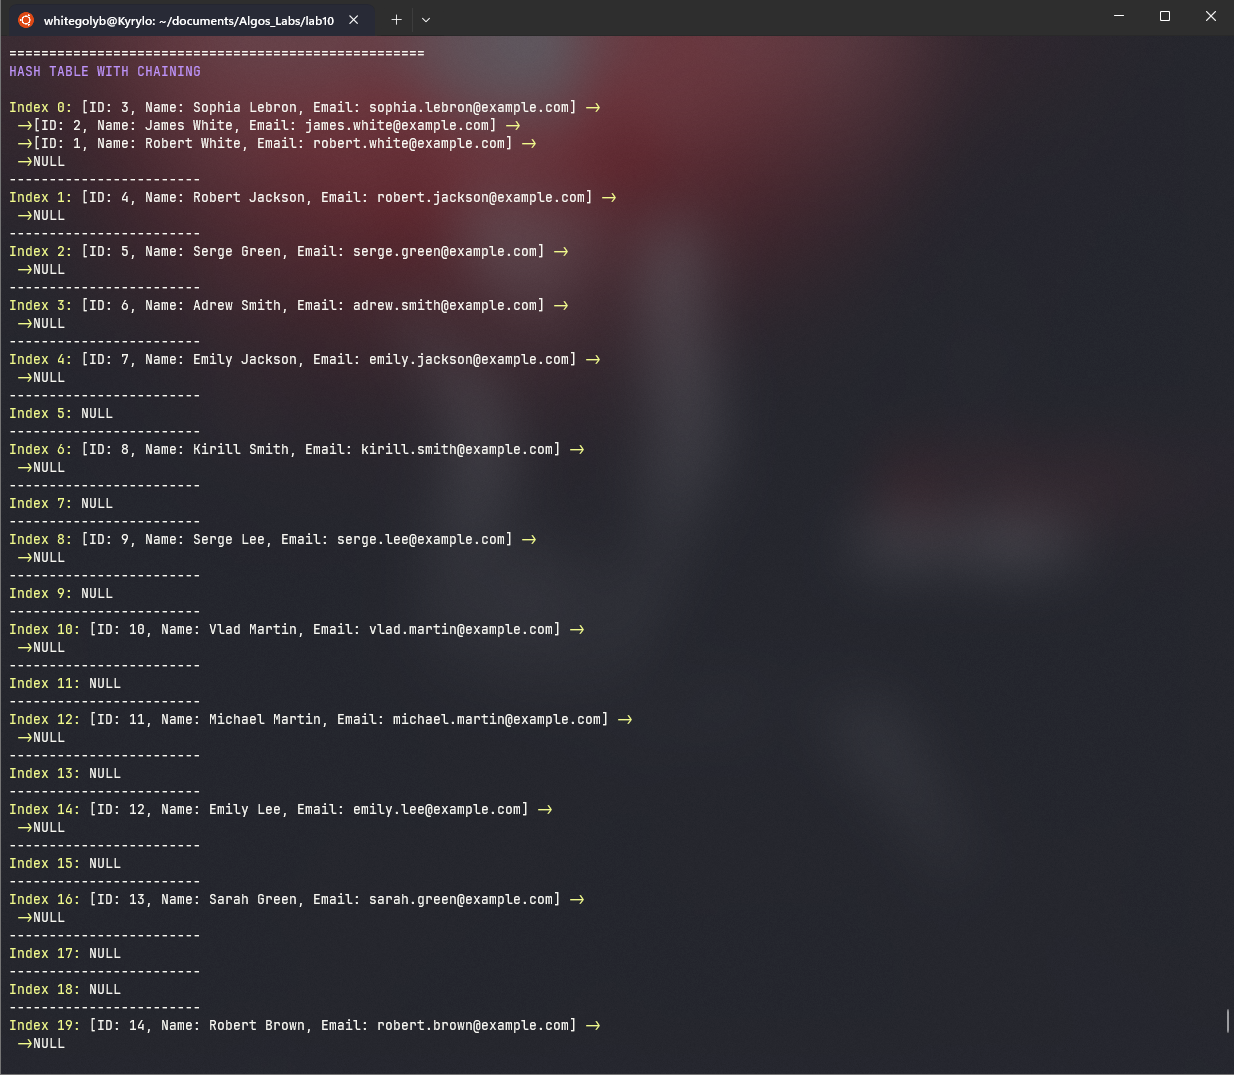
\includegraphics[width=\textwidth]{reports/algos/lab10/assets/1.png}
  \end{subfigure}
  \hfill
  \begin{subfigure}[t]{0.45\textwidth}
      \centering
      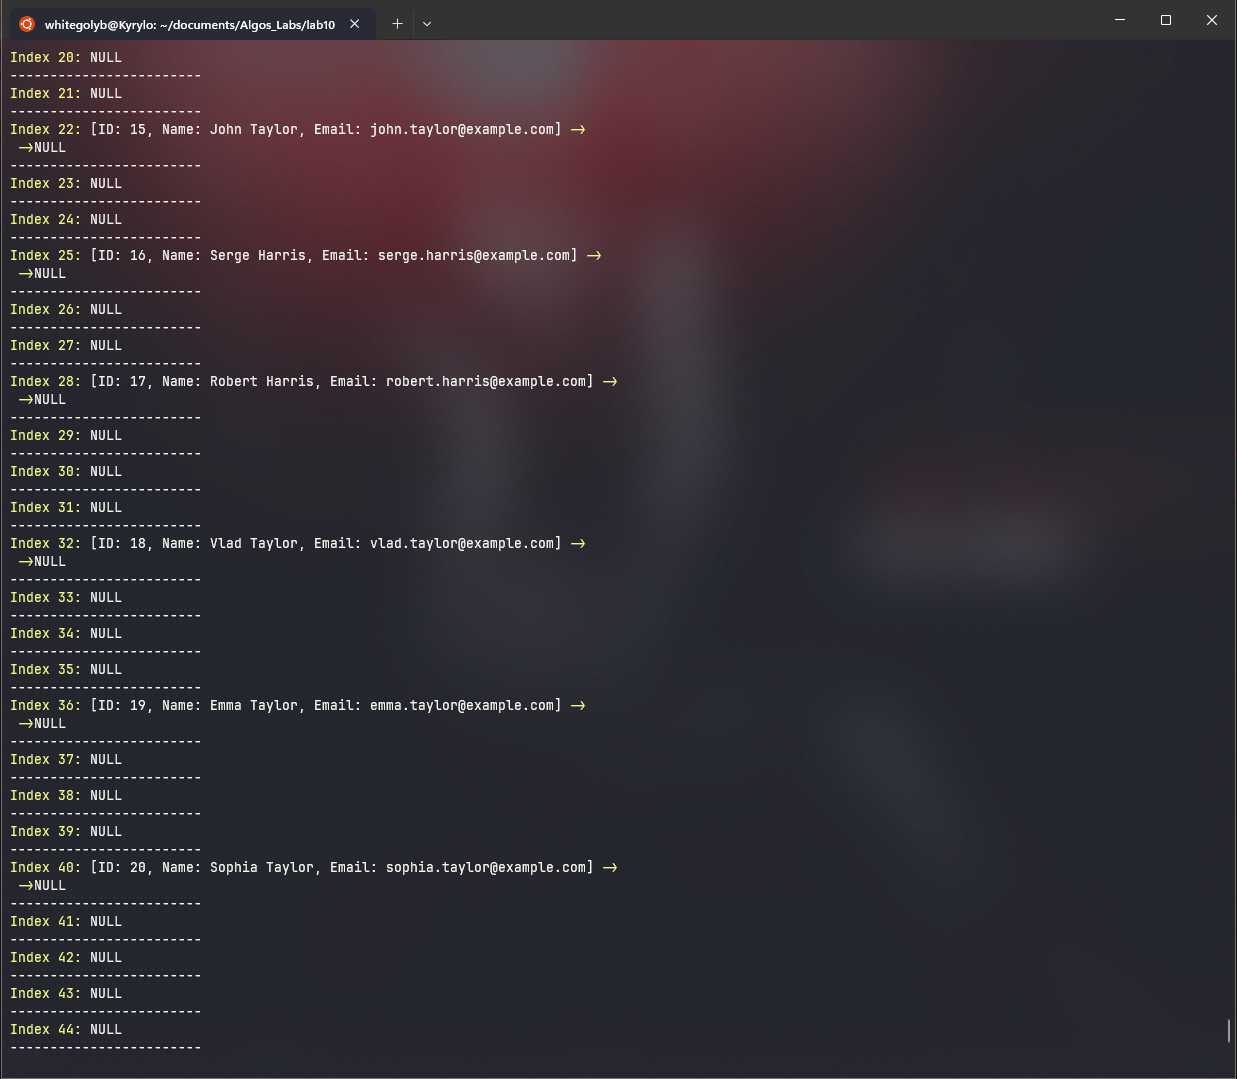
\includegraphics[width=\textwidth]{reports/algos/lab10/assets/2.png}
  \end{subfigure}
  
  \begin{subfigure}[t]{0.45\textwidth}
      \centering
      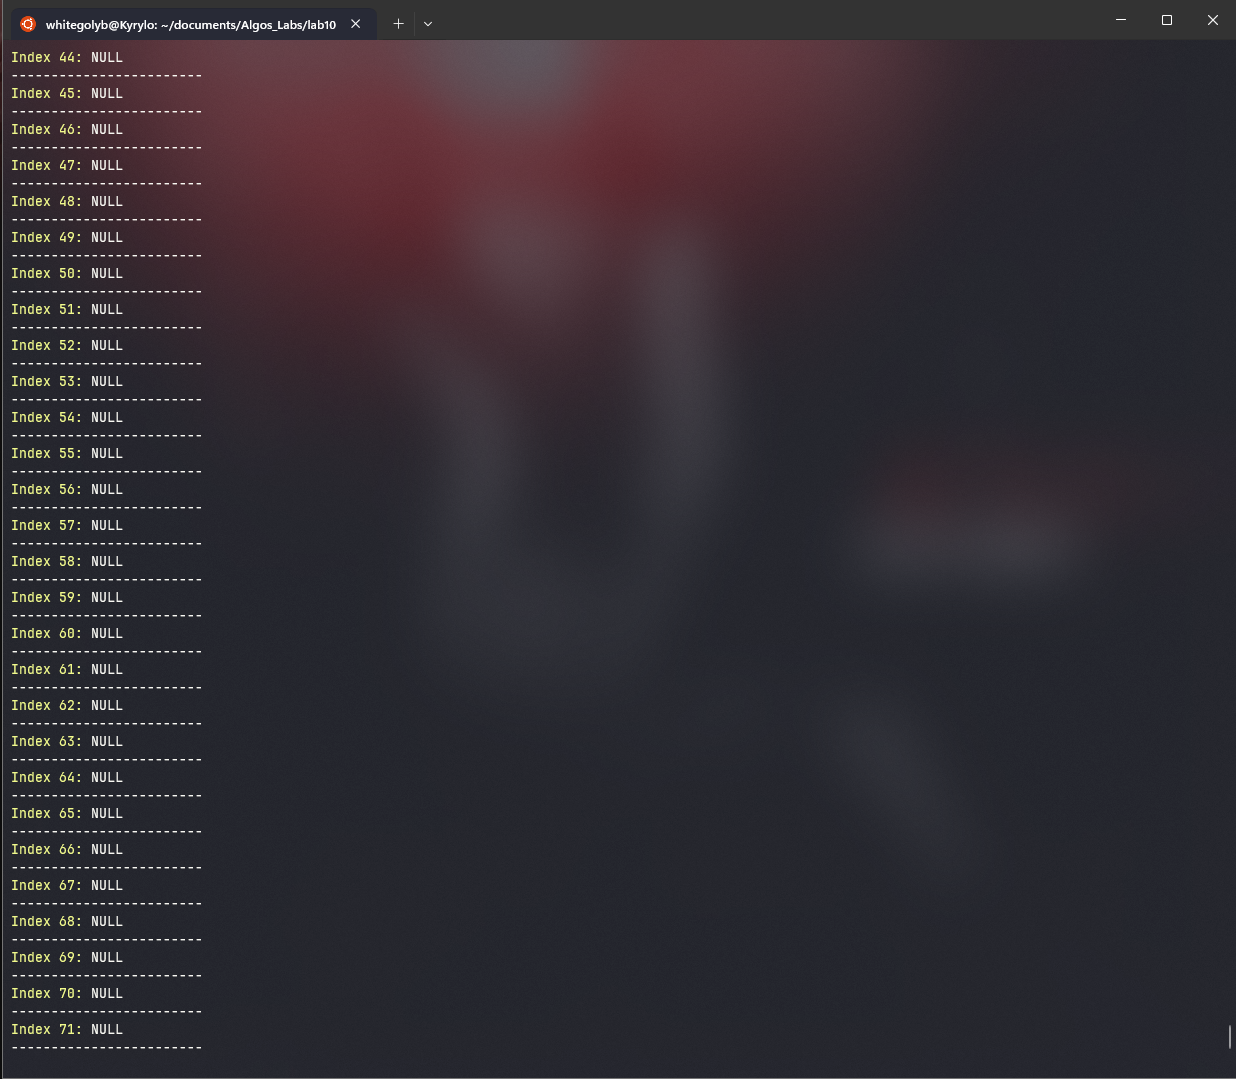
\includegraphics[width=\textwidth]{reports/algos/lab10/assets/3.png}
  \end{subfigure}
  \hfill
  \begin{subfigure}[t]{0.45\textwidth}
      \centering
      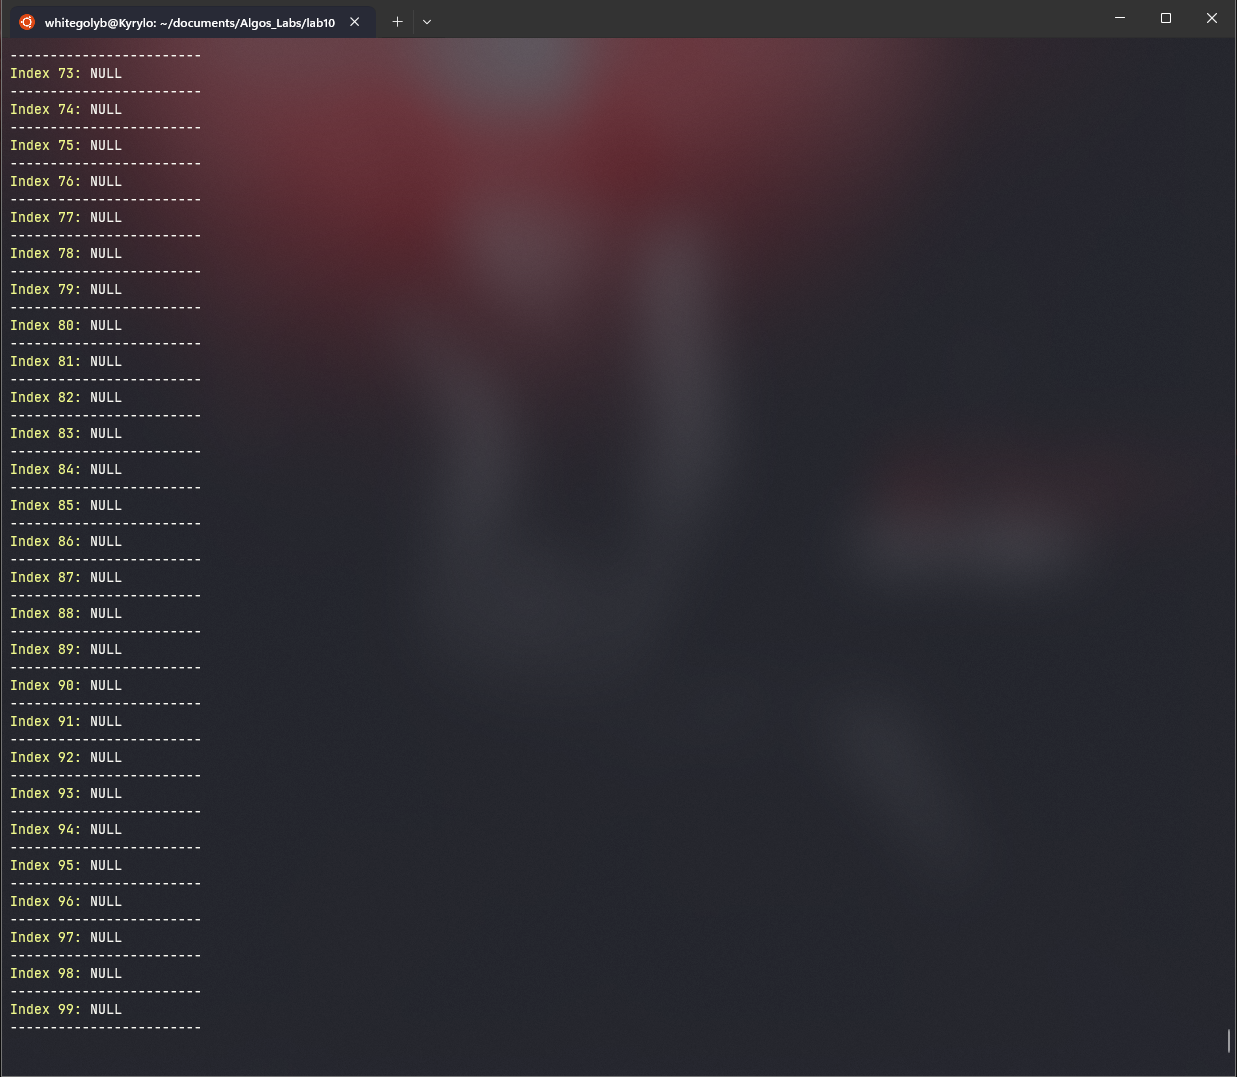
\includegraphics[width=\textwidth]{reports/algos/lab10/assets/4.png}
  \end{subfigure}
  
  \caption{Створена таблиця для 20 елементів, розмір таблиці 100}
\end{figure}

\begin{figure}[h!]
  \centering
  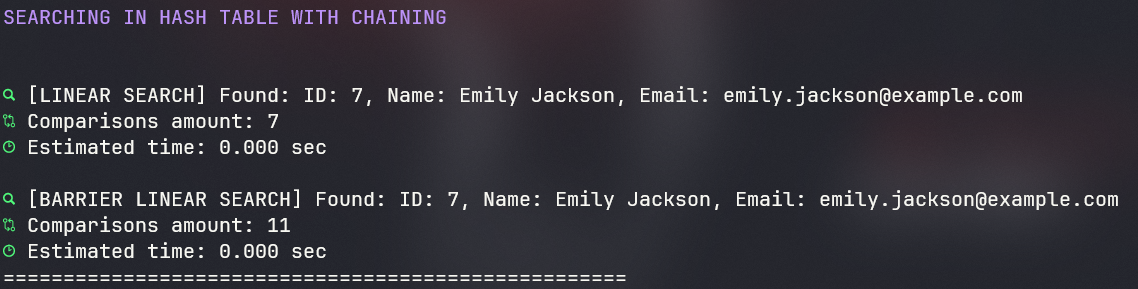
\includegraphics[width=15cm]{reports/algos/lab10/assets/s1.png}
  \caption{Пошуковий результат}
\end{figure}

\begin{figure}[h!]
  \centering
  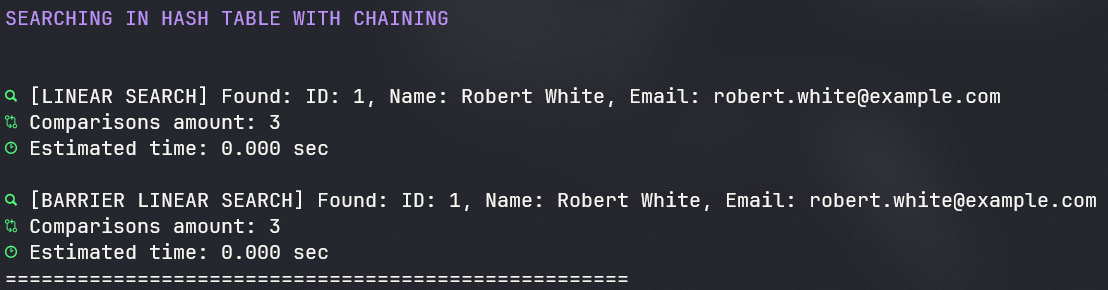
\includegraphics[width=15cm]{reports/algos/lab10/assets/s2.png}
  \caption{Пошуковий результат}
\end{figure}

\begin{figure}[h!]
  \centering
  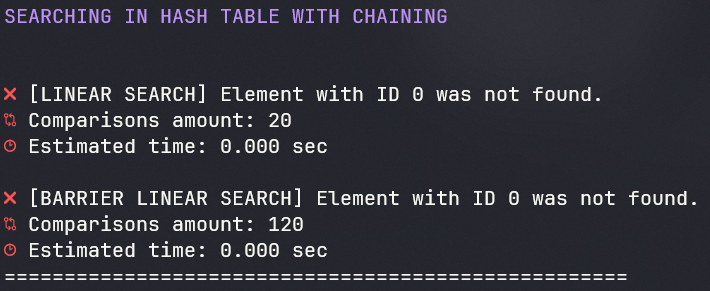
\includegraphics[width=15cm]{reports/algos/lab10/assets/s3.png}
  \caption{Пошуковий результат}
\end{figure}

\begin{figure}[h!]
  \centering
  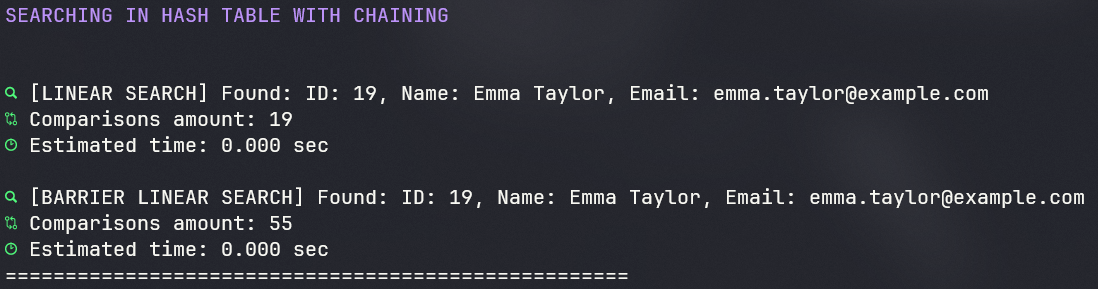
\includegraphics[width=15cm]{reports/algos/lab10/assets/s4.png}
  \caption{Пошуковий результат}
\end{figure}

\clearpage
\subsubsection{Пошукові результати елементу з ID 10:}
\begin{table}[htbp]
\caption{Таблиця результату для лінійного пошуку}
\begin{tabular}{|l|c|c|c|c|}
\hline
Кількість елементів & 20    & 1000  & 5000  & 50000 \\ \hline
Кількість порівнянь & 20    & 162   & 810   & 6480  \\ \hline
Час пошуку (сек)    & 0,001 & 0,001 & 0,001 & 0,002 \\ \hline
\end{tabular}
\end{table}

\vspace{-10pt} 


\begin{table}[htbp]
\caption{Таблиця результату для лінійного пошуку з бар’єром}
\begin{tabular}{|l|c|c|c|c|}
\hline
Кількість елементів & 20    & 1000  & 5000  & 50000 \\ \hline
Кількість порівнянь & 60    & 172   & 820   & 6490  \\ \hline
Час пошуку (сек)    & 0,001 & 0,001 & 0,002 & 0,005 \\ \hline
\end{tabular}
\end{table}

Графіки побудовані на основі таблиць
\begin{figure}[h!]
  \centering
  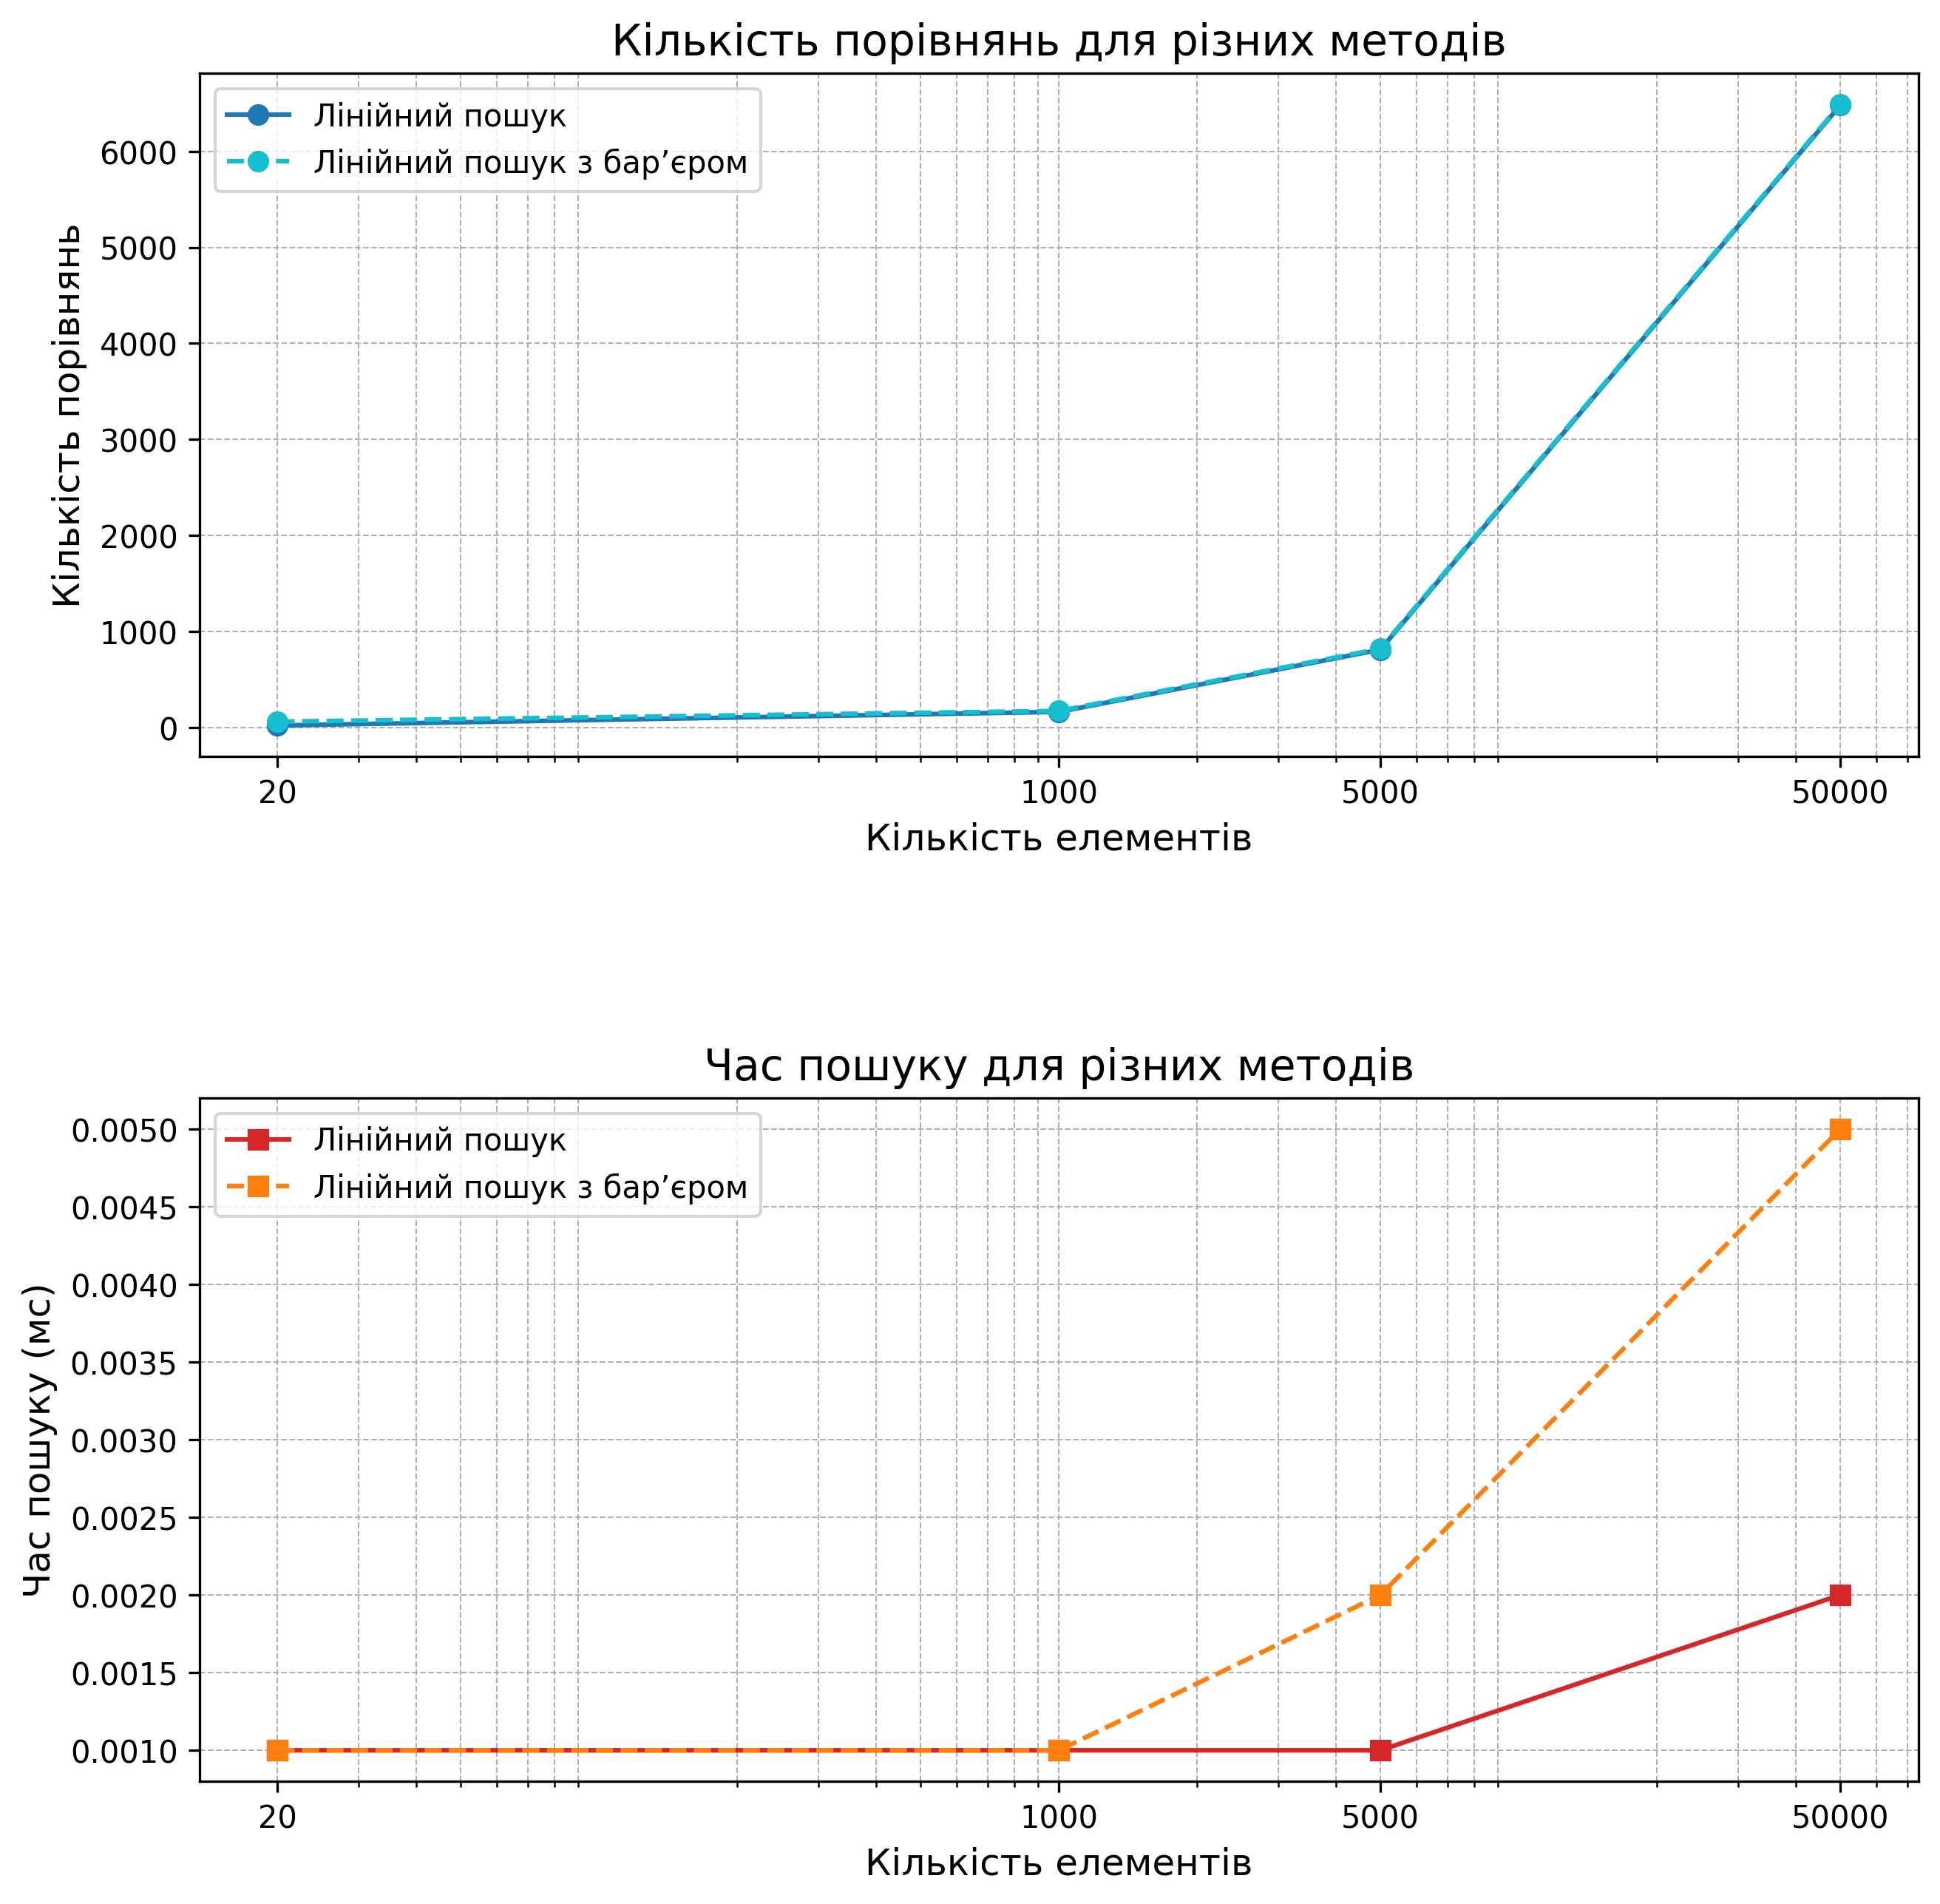
\includegraphics[width=15cm]{reports/algos/lab10/assets/plot.png}
\end{figure}



\clearpage
\section{Висновки}
В ході виконання лабораторної роботи було розроблено два методи пошуку ключа у хеш-таблиці та порівняно їх результати роботи. Порівняння представлено у вигляді таблиць та графіків за параметрами співпадінь та часу виконання відповідно. \\

Можна зазначити що алгоритм з бар`єрами показує гіршу швидкість роботи на більших обсягах даних ніж лінійний, по співпадінням в методів пошуку не дуже велика різниця.\\

Щодо таблиці, вона зберігатиме дані з однаковим хешом у якості списку, що вирішить проблему коллізії, цу можна побачити у розділі результатів.



